\documentclass[a4paper, 11pt]{article}
\usepackage[utf8]{inputenc}
\usepackage[left=1in,right=1in,bottom=0.8in]{geometry}
\usepackage{enumitem}
\usepackage{graphicx}
\graphicspath{ {Figures/} }
\usepackage{float}
\usepackage[labelfont=bf]{caption}
\usepackage{fixltx2e}
\usepackage{caption}
\usepackage{amsmath}
\usepackage{capt-of}
\usepackage{minted}
\usepackage{tabu}
\let\svthefootnote\thefootnote

\title{\bf Experiment 2\\\vspace*{2mm} Combinatorial Circuits Using VHDL\\Two Bit Subtractor}
\author{\it Dhruv Ilesh Shah | 150070016}
\date{January 20, 2017}


\begin{document}
\maketitle
\section*{Overview}
In this lab, I have implemented a combinatorial circuit - the two bit subtractor, using VHDL. Given two input strings of two bits each (say, $x_1x_0$ \& $y_1y_0$), the device computes the difference in modulo 2 sense.

Section 1 contains the approach and main code used for the simulation. Section 2 contains the observations and output of the simulation. For the simulation, I have used GHDL, which is an open-source simulator for the VHDL language.

\section{Setup}

The two bit subtractor is a simple 4-input, 2-output combinatorial circuit. After simplification of the terms, the logic can be given as.
\begin{equation}
\begin{split}
b_0 &= x_0 \oplus y_0 \\
b_1 &= x_1 \oplus y_1 \oplus \overline{x_0}y_0
\end{split}
\end{equation}
As for the implementation, I also 2 intermediate signals $s_1s_0$ defined as below.
\begin{equation}
\begin{split}
s_0 &= x_1 \oplus y_1 \\
s_1 &= \neg x_0 \cdot y_0
\end{split}
\end{equation}
And hence, the final output bit definitions look like:
\begin{equation}
\begin{split}
b_0 &= x_0 \oplus y_0 \\
b_1 &= s_0 \oplus s_1
\end{split}
\end{equation}

This can now be converted to VHDL code and simulated. In this experiment, I have used the \texttt{GenericTB} as testbench, which invokes a DUT entity, and hence the top-level entity would also need to be modified. Defining the DUT entity:

\begin{minted}{vhdl}
entity DUT is
   port(input_vector: in bit_vector(3 downto 0);
       	output_vector: out bit_vector(1 downto 0));
end entity;
\end{minted}

\begin{minted}{vhdl}
architecture DutWrap of DUT is
   component TwoBitSubtractor is
     port(x1,x0,y1,y0: in bit;
         	b1, b0: out bit);
   end component;
begin
   add_instance: TwoBitSubtractor 
			port map (
					x1 => input_vector(3),
					x0 => input_vector(2),
					y1 => input_vector(1),
					y0 => input_vector(0),
					b1 => output_vector(1),
					b0 => output_vector(0));

end DutWrap;
\end{minted}
\hrule
\vspace*{2mm}
Next up, we declare the entity \texttt{TwoBitSubtractor} and its functions. This has been shown below.

\inputminted[linenos]{vhdl}{Submission/TwoBitSubtractor/TwoBitSubtractor.vhd}

\hrule
\vspace*{2mm}
The generic testbench used is also given below.

\inputminted[linenos]{vhdl}{Submission/TwoBitSubtractor/Testbench.vhd}

\hrule
\vspace*{3mm}

For validating, we would need a list of expected values for all the possible input combinations. This can be found as the \texttt{TRACEFILE.txt} below.
\begin{table}[H]
\centering
\begin{tabular}{|c|c|c|}
\hline
$x_1x_0y_1y_0$ & $b_1b_0$ & E\\
\hline
0000 & 00  & 11 \\
0001 & 11  & 11\\
0010 & 10  & 11\\
0011 & 01  & 11\\
0100 & 01  & 11\\
0101 & 00  & 11\\
0110 & 11  & 11\\
0111 & 10  & 11\\
1000 & 10  & 11\\
1001 & 01  & 11\\
1010 & 00  & 11\\
1011 & 11  & 11\\
1100 & 11  & 11\\
1101 & 10  & 11\\
1110 & 01  & 11\\
1111 & 00  & 11\\
\hline
\end{tabular}
\caption{Tracefile for the Two Bit Subtractor}
\end{table}


\section{Observations}

On compiling and executing the \texttt{Testbench}, the circuit was validated with all test cases successful. A snapshot of the same is given below (Figure 1). Test cases and the obtained outputs (ignoring gate delays) can be observed on \texttt{GTKWave} (Figure 2).

\begin{figure}[p]
\centering
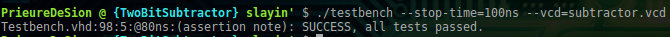
\includegraphics[scale=0.7]{Subtractor_Passed}
\caption{Evaluating Testbench}
\end{figure}

\begin{figure}[p]
\centering
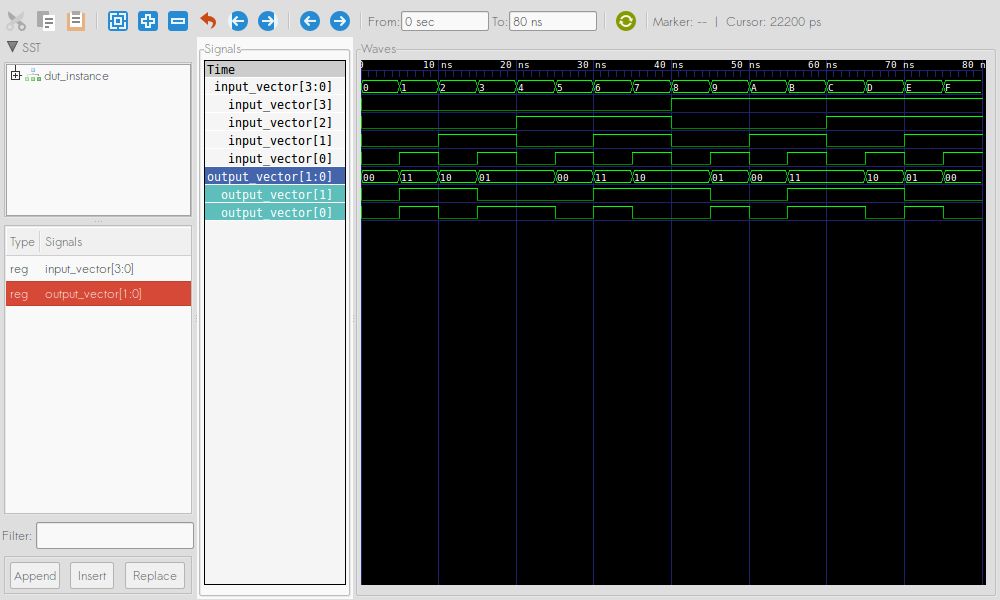
\includegraphics[scale=0.45]{Subtractor_Wave}
\caption{Visualising the waveforms on \texttt{GTKWave}}
\end{figure}

The output file generated by the testbench is given below.
\inputminted{text}{Submission/TwoBitSubtractor/OUTPUTS.txt}

\section*{Conclusion}
Simple combinatorial logic can be implemented and verified very easily by simulating.


\end{document}
